\chapter{Indledning}
\section{Projektformulering}
<<<<<<< HEAD
Interessen for robotteknologi er steget, især indenfor hjælpemidler til ældre. Den aldrende befolkninsgruppe striger stødt, og derfor er der behov for flere 
intelligente løsninger, som kan hjælpe fysisk hæmmede mennesker i deres hverdag. En af ideerne bag dette projekt var konstruktionen af en robot, som kunne hjælpe 
svagelige mennesker med at trække proppen ud af en vinflaske.\\

Smart-produkter er generelt blevet mere udbredte i moderne hjem, og der bliver større krav til hvilke daglige gøremål der skal kunne løses automatisk. Her kunne 
en automatisk vinåbner sætte nye standarder for smart-produkter i almindelige hjem. En sådan vinåbner kunne tilbyde en ny og innoverende måde at åbne en 
vinflaske. Med intelligente enheder som kan detektere vinflaskens postionen og mål, skulle vinåbneren åbne alle typer af vinflasker. \\

Et andet fokuspunkt for vinåbneren er forberedelse af vinen. For at få den optimale oplevelse ud af en vin, skal den åbnes rettidigt så den iltes før indtagelse.
Iltningstiden kan desuden variere fra vin til vin, og derfor kan uerfarne vindrikkere have svært ved at ilte deres vin korrekt. Dette kunne løses ved at 
automatisere denne iltningsprocess, hvor brugeren kan få åbnet vinen til et forudstemt tidspunkt bestemt ud fra vinens type.\\

Derudover kunne den automatiske vinåbner indeholde en række features som kunne forbedre vinoplevelsen. Dette kan gøre den til et tiltrækkende produkt også for 
vinentusiaster, som ønsker et premium produkt der kan give dem en større nydelse ved vindrikning.\\


\section{winePrep}
Visionen for den automatiske vinåbner "winePrep" var et system som kunne imødegå et hvert behov der måtte være indenfor drikning og forberedelse af vin. \\
Udover selve åbningen af en vinflaske skal systemet:\\
- Automatisk kunne finde vinflaskes top, så alle typer vinflasker uanset højde og øvrige mål kunne åbnes.\\ 
- Kunne åbne vinen til et forudbestem tidspunkt og derved sikre en optimal iltning af vinen\\
- Kunne måle vinens temperatur, og regulere denne så vinen kan nydes ved dens optimale betingelser.\\
- Kunne finde information om den optimale iltningstid for en bestemt vin via tilslutning til en database\\
- Indeholde en social medie platform "winebook", hvor brugere kunne anmelde vine, og interagere med andre vinelskere\\
- Have en mobil applikation tilsluttet, der gjorde fjernbetjening af systemet muligt\\
- Kunne scanne etiketten på en vinflakse og finde information om vinen via en database\\
- Kunne dispensere korkproppen for vinflasken efter vinåbningen er afsluttet.\\

Ved udformingen af det ideele produkt er der ikke taget hensyn til gruppens begrænsede tid, ressourcer og kompetencer. Visionen for winePrep fungere
i dette projekt blot som et startsted for det videre projektforløb. Ud fra det ideelle produkt vil gruppen udvælge de funktioner som vurderes til realistisk
set at kunne gennemføres. 
=======
Mange ældre har i dag svært ved at åbne deres vinflaske, da de ikke har den fornødne styrke til selv at trække korkproppen ud af vinflasken. Derfor vil det være ideelt for dem, at have en løsning hvor åbningen af vinflaskerne bliver automatiseret.

For at få den optimale oplevelse ud af en vin, skal den åbnes rettidigt så den iltes før indtagelse. Iltningstiden kan variere fra vin til vin, og derfor kan mange uerfarne vindrikkere have svært ved at ilte deres vin korrekt. Mange glemmer at åbne vinen i god tid, og opnår derfor ikke den optimale oplevelse. Det kan derfor være ideelt, hvis denne proces også automatiseres.

\begin{figure}[H]
	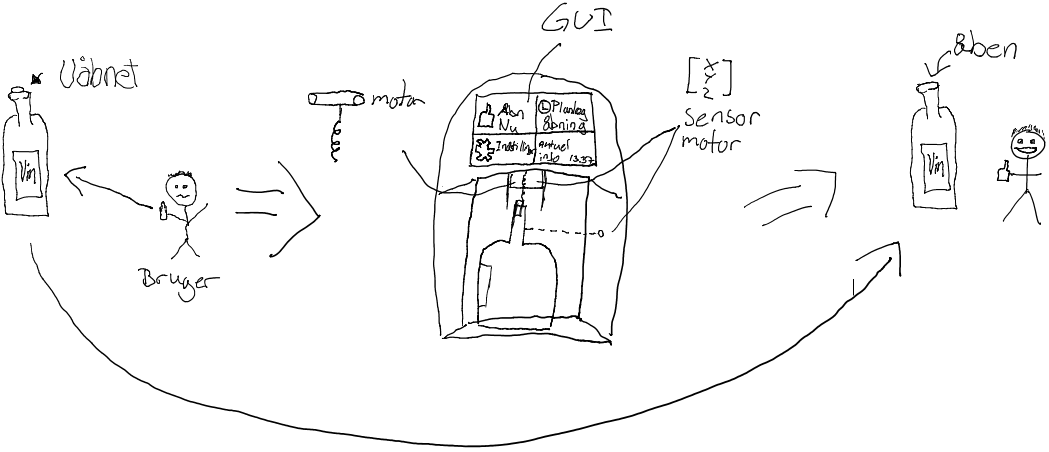
\includegraphics[scale=0.6]{WinePrep_realistisk.png}
	\caption{Rigt billede der beskriver WinePrep}
	\label{RIGTBILLEDE}
\end{figure}

\section{Det realistiske system}
WinePrep er den automatiske vinåbner som er illustreret på Figur \ref{RIGTBILLEDE}, hvilket beskriver det realistiske system i en tænkt situation. Der er siden udarbejdelsen af det rige billede ikke ændret ved tanken bag systemets funktionalitet, blot andre måder at implementere ideerne på.\\

Den oprindelige tanke med WinePrep gør det for brugeren muligt at åbne en bestemt type vinflaske ved at indsætte vinen i maskinen, konfigurere WinePrep til at åbne og derefter først lade systemet lokalisere flasken hvorefter en åbningsmekanisme sænker sig over vinen og trækker korkproppen op. Dette realiseres med WinePreps ramme, brugergrænseflade, sensorer, aktuatorer og proptrækker samt microcontrollere til at lade systemet kommunikere internt.

På baggrund af de tekniske komponenter og WinePreps kompleksitet, vil der til udviklere være krav om forhåndskendskab til elektronik og programmering, på et plan der gør det muligt at forstå og bruge de oplysninger der findes i bilagene til denne rapport.

WinePrep er en prototype der er mulig at udvikle og optimere på.

\section{Hovedansvarsområder}
Tabel xx viser fordelingen af hovedansvarsområder for produktet fordelt på gruppemedlemmer. Emnerne er inddelt i primær og sekundær, som informerer om medlemmers specialistviden og kernekompetencer indenfor produktudviklingen. Enkelte sekundære felter er tomme, dette betyder at ingen har været sekundær på emnet.\\

\begin{tabular}{| l | c | c |}
\hline
Emne & Primær & Sekundær\\\hline
Brugergrænseflade (GUI) & AS & HVB\\\hline
SPI DevKit-PSoC & HVB & JMH\\\hline
SPI PSoC-PSoC & HVB, JMH & \\\hline
PSoC software sensor & JMH & MBE\\\hline
PSoC software sensor & JMH & MBE\\\hline
Bipolære motorer & MBE & JMH\\\hline
Unipolære motorer & MBE & JMH\\\hline
DC motor & MBE & \\\hline
Konstruktion og mekanik & AS & HVB\\\hline
\end{tabular}
>>>>>>> 35b9baa5efe9247fbd2bc55cc1310ffe96b449b9
